\documentclass[12pt]{../vespers-sheet} %booklet
\usepackage{multicol}

\begin{document}

% TODO: Update the title for the specific feast
\chapter*{Solemn First Vespers of the Assumption of the Blessed Virgin Mary}

\begin{center}
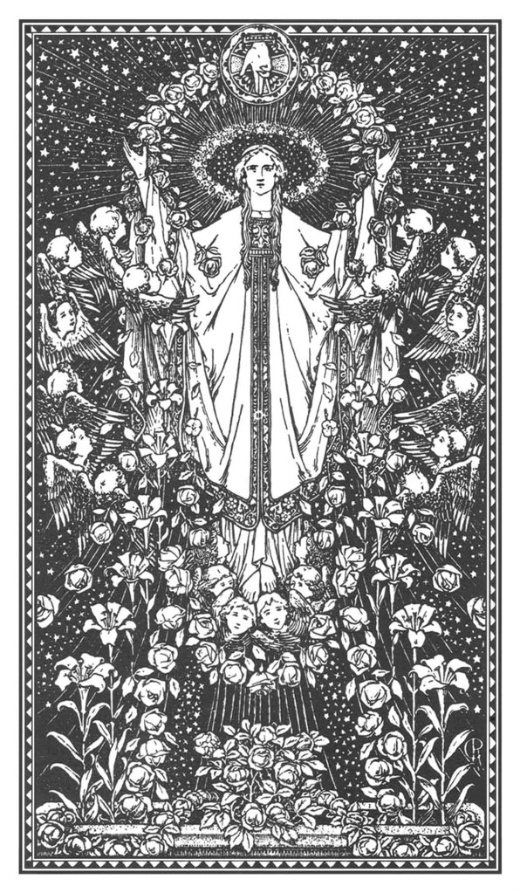
\includegraphics[width=0.55\textwidth]{AssumptionVirgoMaria}
\end{center}

\vfill\pagebreak

%\section*{Beginning of the Office}

\begin{rubricbox}

{\color{red}When the Officiant kneels, all \textbf{kneel} and pray silently.
Then, when the Officiant stands, all \textbf{stand} and say silently one \textit{Pater noster} (Our Father) and \textit{Ave Maria} (Hail Mary).
Then all make the sign of the cross with the Officiant as he intones:}

\end{rubricbox}

% TODO: Make sure that the tone of the deus adjutorium matches the season primarily and the solemnity of the feast secondarily
 \gresetinitiallines{1}
\gregorioscore{../common/deus-in-adjutorium-solemn}

\textit{
O God, come to my assistance.
{\color{red}\Vbar.}~O Lord, make haste to help me.
Glory be to the Father, and to the Son, and to the Holy Spirit,
as it was in the beginning, is now, and ever shall be, world without end. Amen.
Praise to Thee, O Lord, King of endless glory.}

%\vfill\pagebreak

\section*{Psalm 109}

\textit{\textnormal{Ant. 1.} Mary is taken up into Heaven, the Angels rejoice, and bless God with songs of praise.
 \textnormal{Ps.} The Lord said to my lord, sit thou at My right hand.}

\gresetinitiallines{1}
\gregorioscore{ps109-antiphon}

\gresetinitiallines{0}
\gregorioscore{ps109-intonation}

 \begin{latinenglishsection}

\latinenglish{

	2. Donec ponam ini\textbf{mí}cos \textbf{tu}os,~* scabéllum \textbf{pe}dum tu\textbf{ó}rum.

3. Virgam virtútis tuæ emíttet Dómi\textbf{nus} ex \textbf{Si}on:~* domináre in médio inimi\textbf{có}rum tu\textbf{ó}rum.

4. Tecum princípium in die virtútis tuæ in splendóri\textbf{bus} sanc\textbf{tó}rum:~* ex útero ante lucíferum \textbf{gé}nu\textbf{i} te.

5. Jurávit Dóminus, et non pœni\textbf{té}bit \textbf{e}um:~* Tu es sacérdos in ætérnum secúndum órdi\textbf{nem} Mel\textbf{chí}sedech.

6. Dóminus a \textbf{dex}tris \textbf{tu}is,~* confrégit in die iræ \textbf{su}æ \textbf{re}ges.

7. Judicábit in natiónibus, im\textbf{plé}bit ru\textbf{í}nas:~* conquassábit cápita in \textbf{ter}ra mul\textbf{tó}rum.

8. De torrénte in \textbf{vi}a \textbf{bi}bet:~* proptérea exal\textbf{tá}bit \textbf{ca}put.

9. {\color{red}\textit{(bow)}} Glória \textbf{Pa}tri, et \textbf{Fí}\textbf{li}o,~* et Spi\textbf{rí}tui \textbf{Sanc}to.

10. {\color{red}\textit{(rise)}} Sicut erat in princípio, et \textbf{nunc}, et \textbf{sem}per,~* et in s\'{\ae}cula sæcu\textbf{ló}rum. \textbf{A}men. %% 

}{
	% 1. The Lord said to my Lord: Sit thou at my right hand:

2. Until I make thy enemies thy footstool.
 
3. The Lord will send forth the sceptre of thy power out of Sion: rule thou in the midst of thy enemies.
 
4. With thee is the principality in the day of thy strength: in the brightness of the saints:
 from the womb before the day star I begot thee.
 
5. The Lord hath sworn, and he will not repent: Thou art a priest for ever according to the order of Melchisedech.
 
6. The Lord at thy right hand hath broken kings in the day of his wrath.

7. He shall judge among nations, he shall fill ruins: he shall crush the heads in the land of the many.

8. He shall drink of the torrent in the way: therefore shall he lift up the head. 

Glory be. %%
}

\end{latinenglishsection}

\gresetinitiallines{1}
\gregorioscore{ps109-antiphon}

%%

\section*{Psalm 112}

\textit{\textnormal{Ant. 2.} The Virgin Mary is taken up into the bridal chamber of heaven, where the King of kings sitteth on His starry throne.
 \textnormal{Ps.} Praise the Lord, ye children: praise ye the name of the Lord.}

\gresetinitiallines{1}
\gregorioscore{ps112-antiphon}

\gresetinitiallines{0}
\gregorioscore{ps112-intonation}

 \begin{latinenglishsection}

\latinenglish{

	2. Sit nomen Dómi\textit{ni} \textit{be}\textit{ne}\textbf{díc}tum,~* 
	ex hoc nunc, et us\textit{que} \textit{in} \textbf{s\'{\ae}}culum.

3. A solis ortu us\textit{que} \textit{ad} \textit{oc}\textbf{cá}sum,~* 
	laudábile \textit{no}\textit{men} \textbf{Dó}mini.

4. Excélsus super om\textit{nes} \textit{gen}\textit{tes} \textbf{Dó}minus,~* 
	et super cælos gló\textit{ri}\textit{a} \textbf{e}jus.

5. Quis sicut Dóminus, Deus noster, qui \textit{in} \textit{al}\textit{tis} \textbf{há}bitat,~* 
	et humília réspicit in cælo \textit{et} \textit{in} \textbf{ter}ra?

6. Súscitans \textit{a} \textit{ter}\textit{ra} \textbf{ín}opem,~* 
	et de stércore é\textit{ri}\textit{gens} \textbf{páu}perem:

7. Ut cóllocet e\textit{um} \textit{cum} \textit{prin}\textbf{cí}pibus,~* 
	cum princípibus pó\textit{pu}\textit{li} \textbf{su}i.

8. Qui habitáre facit sté\textit{ri}\textit{lem} \textit{in} \textbf{do}mo,~* 
	matrem filió\textit{rum} \textit{læ}\textbf{tán}tem.

9. {\color{red}\textit{(bow)}} Glória \textit{Pa}\textit{tri}, \textit{et} \textbf{Fí}lio,~* 
	et Spirí\textit{tu}\textit{i} \textbf{Sanc}to.

10. {\color{red}\textit{(rise)}} Sicut erat in princípio, \textit{et} \textit{nunc}, \textit{et} \textbf{sem}per,~* 
	et in s\'{\ae}cula sæcu\textit{ló}\textit{rum}. \textbf{A}men. %%

}{
	%1. Praise the Lord, ye children: praise ye the name of the Lord.
 	
2. Blessed be the name of the Lord, from henceforth now and for ever.
 	
3. From the rising of the sun unto the going down of the same, the name of the Lord is worthy of praise.
 	
4. The Lord is high above all nations; and his glory above the heavens.
 	
5.Who is as the Lord our God, who dwelleth on high, and looketh down on the low things in heaven and in earth?
 	
6. Raising up the needy from the earth, and lifting up the poor out of the dunghill:
 	
7. That he may place him with princes, with the princes of his people.
 	
8. Who maketh a barren woman to dwell in a house, the joyful mother of children. 

Glory be. %%
}

\end{latinenglishsection}

\gresetinitiallines{1}
\gregorioscore{ps112-antiphon}

%%

\section*{Psalm 121}

\textit{\textnormal{Ant. 3.} We run after the odour of Thine ointments. The young maidens have loved thee exceedingly.
 \textnormal{Ps.} I rejoiced at the things that: were said to me: We shall go into the house of the Lord.}

\gresetinitiallines{1}
\gregorioscore{ps121-antiphon}

\gresetinitiallines{0}
\gregorioscore{ps121-intonation}

 \begin{latinenglishsection}

\latinenglish{

	2. Stantes e\textit{rant} \textit{pe}\textit{des} \textbf{nos}tri,~* 
	in átriis \textit{tu}\textit{is}, \textit{Je}\textbf{rú}salem.

3. Jerúsalem, quæ ædifi\textit{cá}\textit{tur} \textit{ut} \textbf{cí}vitas:~*
	cujus participátio e\textit{jus} \textit{in} \textit{id}\textbf{íp}sum.

4. Illuc enim ascendérunt tri\textit{bus}, \textit{tri}\textit{bus} \textbf{Dó}mini:~*
	testimónium Israël ad confiténdum \textit{nó}\textit{mi}\textit{ni} \textbf{Dó}mini.

5. Quia illic sedérunt se\textit{des} \textit{in} \textit{ju}\textbf{dí}cio,~*
	sedes su\textit{per} \textit{do}\textit{mum} \textbf{Da}vid.

6. Rogáte quæ ad pa\textit{cem} \textit{sunt} \textit{Je}\textbf{rú}salem:~*
	et abundántia di\textit{li}\textit{gén}\textit{ti}\textbf{bus} te:

7. Fiat pax in \textit{vir}\textit{tú}\textit{te} \textbf{tu}a:~*
	et abundántia in \textit{túr}\textit{ri}\textit{bus} \textbf{tu}is.

8. Propter fratres meos, et \textit{pró}\textit{xi}\textit{mos} \textbf{me}os,~* 
	loqué\textit{bar} \textit{pa}\textit{cem} \textbf{de} te:

9. Propter domum Dómi\textit{ni}, \textit{De}\textit{i} \textbf{nos}tri,~* 
	quæsí\textit{vi} \textit{bo}\textit{na} \textbf{ti}bi.

10. {\color{red}\textit{(bow)}} Glória \textit{Pa}\textit{tri}, \textit{et} \textbf{Fí}lio,~*
	et Spi\textit{rí}\textit{tu}\textit{i} \textbf{Sanc}to.

11. {\color{red}\textit{(rise)}} Sicut erat in princípio, \textit{et} \textit{nunc}, \textit{et} \textbf{sem}per,~*
	et in s\'{\ae}cula sæ\textit{cu}\textit{ló}\textit{rum}. \textbf{A}men.
	 %%

}{
	%1. I rejoiced at the things that were said to me: We shall go into the house of the Lord.

2. Our feet were standing in thy courts, O Jerusalem.

3. Jerusalem, which is built as a city, which is compact together.

4. For thither did the tribes go up, the tribes of the Lord: the testimony of Israel, to praise the name of the Lord.

5. Because their seats have sat in judgment, seats upon the house of David.

6. Pray ye for the things that are for the peace of Jerusalem: and abundance for them that love thee.

7. Let peace be in thy strength: and abundance in thy towers.

8. For the sake of my brethren, and of my neighbours, I spoke peace of thee.

9. Because of the house of the Lord our God, I have sought good things for thee.

Glory be.  %%
}

\end{latinenglishsection}

\gresetinitiallines{1}
\gregorioscore{ps121-antiphon}

%%

\section*{Psalm 126}

\textit{\textnormal{Ant. 4.} O Daughter, blessed art thou of the Lord, for through thee we have partaken of the fruit of life.
 \textnormal{Ps.} Unless the Lord build the house, they labour in vain that build it.}

\gresetinitiallines{1}
\gregorioscore{ps126-antiphon}

\gresetinitiallines{0}
\gregorioscore{ps126-intonation}

 \begin{latinenglishsection}

\latinenglish{

	2. Nisi Dóminus custodíerit \textbf{ci}vi\textbf{tá}tem,~* 
	frustra vígilat qui cus\textbf{tó}dit \textbf{e}am.

3. Vanum est vobis ante \textbf{lu}cem \textbf{súr}\textbf{ge}re:~* 	
	súrgite postquam sedéritis, qui manducátis \textbf{pa}nem do\textbf{ló}ris.

4. Cum déderit diléctis \textbf{su}is \textbf{som}num:~*	
	ecce heréditas Dómini fílii: merces, \textbf{fruc}tus \textbf{ven}tris.

5. Sicut sagíttæ in \textbf{ma}nu pot\textbf{én}tis:~* 
	ita fílii \textbf{ex}cus\textbf{só}rum.

6. Beátus vir qui implévit desidérium \textbf{su}um ex \textbf{ip}sis:~*
	non confundétur cum loquétur inimícis \textbf{su}is in \textbf{por}ta.

7. {\color{red}\textit{(bow)}} Glória \textbf{Pa}tri, et \textbf{Fí}\textbf{li}o,~*
	et Spi\textbf{rí}tui \textbf{Sanc}to.

8. {\color{red}\textit{(rise)}} Sicut erat in princípio, et \textbf{nunc}, et \textbf{sem}per,~* 
	et in s\'{\ae}cula sæcu\textbf{ló}rum. \textbf{A}men. %%

}{
	%1. Unless the Lord build the house, they labour in vain that build it.

2. Unless the Lord keep the city, he watcheth in vain that keepeth it.

3. It is vain for you to rise before light, rise ye after you have rested, you that eat the bread of sorrow.

4. When he shall give sleep to his beloved: behold the inheritance of the Lord are children: the reward, the fruit of the womb.

5. As arrows in the hand of the mighty, so the children of them that have been cast out.

6. Blessed is the man that hath filled his desire with them;
he shall not be confounded when he shall speak to his enemies in the gate. 

Glory be. %%
}

\end{latinenglishsection}

\gresetinitiallines{1}
\gregorioscore{ps126-antiphon}

%%

\section*{Psalm 147}

\textit{\textnormal{Ant. 5.} Fair and beautiful art thou, O daughter of Jersualem, terrible as an army in battle array.
 \textnormal{Ps.} Praise the Lord, O Jerusalem: praise thy God, O Sion.}

\gresetinitiallines{1}
\gregorioscore{ps147-antiphon}

\gresetinitiallines{0}
\gregorioscore{ps147-intonation}

 \begin{latinenglishsection}

\latinenglish{

	2. Quóniam confortávit seras por\textit{tá}\textit{rum} \textit{tu}\textbf{á}rum:~* 
	benedíxit fíliis \textit{tu}\textit{is} \textbf{in} te.

3. Qui pósuit fi\textit{nes} \textit{tu}\textit{os} \textbf{pa}cem:~* 
	et ádipe fruménti \textit{sá}\textit{ti}\textbf{at} te.

4. Qui emíttit elóqui\textit{um} \textit{su}\textit{um} \textbf{ter}ræ:~* 
	velóciter currit \textit{ser}\textit{mo} \textbf{e}jus.

5. Qui dat ni\textit{vem} \textit{sic}\textit{ut} \textbf{la}nam:~* 
	nébulam sicut cí\textit{ne}\textit{rem} \textbf{spar}git.

6. Mittit crystállum suam \textit{sic}\textit{ut} \textit{buc}\textbf{cél}las:~* 
	ante fáciem frígoris ejus quis \textit{sus}\textit{ti}\textbf{né}bit?

7. Emíttet verbum suum, et lique\textit{fá}\textit{ci}\textit{et} \textbf{e}a:~* 
	flabit spíritus ejus, et \textit{flu}\textit{ent} \textbf{a}quæ.

8. Qui annúntiat ver\textit{bum} \textit{su}\textit{um} \textbf{Ja}cob:~* 
	justítias, et judícia \textit{su}\textit{a} \textbf{Is}raël.

9. Non fecit táliter om\textit{ni} \textit{na}\textit{ti}\textbf{ó}ni:~* 
	et judícia sua non manifes\textit{tá}\textit{vit} \textbf{e}is.

10. {\color{red}\textit{(bow)}} Glória \textit{Pa}\textit{tri}, \textit{et} \textbf{Fí}\textbf{li}o,~* 
	et Spirí\textit{tu}\textit{i} \textbf{Sanc}to.

11. {\color{red}\textit{(rise)}} Sicut erat in princípio, \textit{et} \textit{nunc}, \textit{et} \textbf{sem}per,~* 
	et in s\'{\ae}cula sæcu\textit{ló}\textit{rum}. \textbf{A}men. %%

}{
	%1. Praise the Lord, O Jerusalem: praise thy God, O Sion.

2. Because he hath strengthened the bolts of thy gates, he hath blessed thy children within thee.

3. Who hath placed peace in thy borders: and filleth thee with the fat of corn.

4. Who sendeth forth his speech to the earth: his word runneth swiftly.

5. Who giveth snow like wool: scattereth mists like ashes.

6. He sendeth his crystal like morsels: who shall stand before the face of his cold?

7. He shall send out his word, and shall melt them: his wind shall blow, and the waters shall run.

8. Who declareth his word to Jacob: his justices and his judgments to Israel.

9. He hath not done in like manner to every nation: and his judgments he hath not made manifest to them.

Glory be. %%
}

\end{latinenglishsection}

\gresetinitiallines{1}
\gregorioscore{ps147-antiphon}

%%

\section*{Little Chapter (Judith 13:22-23)}

\textit{\color{red}The Officiant leads the Little Chapter:}

\begin{latinenglishsection}

\latinenglish{
	Benedíxit te Dóminus in virtúte sua, quia per te ad níhilum redégit inimícos \textbf{no}stros. {\color{red}\GreDagger}\ Benedícta es tu, fília, a Dómino De\textit{o ex}\textbf{cél}so, præ ómnibus muliéribus super \textbf{ter}ram.
	{\color{red}\Rbar.}~Deo grátias.
}{
	The Lord hath blessed thee by his power, because by thee he hath brought our enemies to nought. Blessed art thou, O daughter, by the Lord the most high God, above all women upon the earth.
	 {\color{red}\Rbar.}~Thanks be to God.
}

\end{latinenglishsection}

% TODO: Verify that the hymn is correct for the feast (including the responsory after the hymn)

\section*{Hymn}

\textit{\color{red}The Cantor leads the hymn:}

\gresetinitiallines{1}
\gregorioscore{../hymns/o-prima-virgo}

{\itshape

	1.  O Virgin thou, the spirit's fair'st,
	Predestined by the will divine,
	Within thy sacred womb thou bear'st
	His only Son, and also thine.
	
	2. O thou in whom rich grace abounds,
	Foretold thou wast to be the foe
	Who in her origin confounds
	The wicked demon here below.
	
	3. Within thy womb anew Life's made,
	The very life by Adam lost
	Has been renewed by thee, sweet maid,
	Who didst provide the holocaust.
	
	4. Thy will immersed in Jesus' own,
	Atoning for the sins of all,
	He raises thee to Heaven's throne,
	In victory o'er death's dread thrall.
	
	5. In thy great glory burning bright
	Exalted nature sings the praise,
	And unto beauty's very height,
	Dost honor and all glory raise.
	
	6. Triumphant Queen to Heaven borne,
	Upon us exiles turn thy sight,
	That to the ever-blessed morn
	We may be guided by thy light.
	
	7. All honor, laud, and glory be,
	O Jesu, Virgin-born to thee;
	All glory, as is ever meet
	To Father and to Paraclete.
	Amen.
}

\textit{\color{red}The Cantor says the following before all reply afterwards:}

\gresetinitiallines{0}
\gabcsnippet{
(c3) <c><sp>V/</sp>.</c> Ex(h)al(h)tá(hi)ta(h) est(h') (,) sanc(h)ta(h) De(f')i(e) Gé(fh_)ni(h)trix.(hi/H'/G'/hi/h.gh/G'FE'/fg/gf.) (::)
}

\gresetinitiallines{0}
\gabcsnippet{
(c3) <c><sp>R/</sp>.</c> Su(h)per(h) cho(h)ros(h) An(h)ge(h)ló(hi)rum(h') (,) ad(h) cæ(h)lés(h)ti(f')a(e) re(fh_)gna.(hi/H'/G'/hi/h.gh/G'FE'/fg/gf.)(::)
}

\textit{{\color{red}\Vbar.}~The holy Mother of God hath been exalted.
{\color{red}\Rbar.}~Over choirs of Angels, into the heavenly kingdom.}

%TODO: Verify that the magnificat antiphon is correct and match the mangificat intonation and pointed text with the tone

\section*{Magnificat}

\textit{\textnormal{Ant Magn.} O Virgin most prudent, whither goest thou, like the golden dawn? Daughter of Sion, thou art all beautiful and sweet; fair as the moon, bright as the sun.
\textnormal{Cant.} My soul doth magnify the Lord: and my spirit hath rejoiced in God my Saviour.}

\begin{rubricbox}

{\color{red}The Cantor leads by intoning the antiphon and the first verse.}

\end{rubricbox}

\gresetinitiallines{1}
\gregorioscore{magnificat-antiphon-only}

\begin{rubricbox}

{\color{red}All \textbf{stand} and make the sign of the cross with the Cantor.}

\end{rubricbox}

\gresetinitiallines{0}
\gregorioscore{magnificat-intonation}

 \begin{latinenglishsection}

\latinenglish{	
	3. Quia respéxit humilitátem \textit{an}\textit{cíl}\textit{læ} \textbf{su}æ:~* 
ecce enim ex hoc beátam me dicent omnes gene\textit{ra}\textit{ti}\textbf{ó}nes.

	4. Quia fecit mihi \textit{ma}\textit{gna} \textit{qui} \textbf{pot}\textbf{ens} est:~* 
	et sanctum \textit{no}\textit{men} \textbf{e}jus.

	5. Et misericórdia ejus a progéni\textit{e} \textit{in} \textit{pro}\textbf{gé}\textbf{ni}es~* 
	timén\textit{ti}\textit{bus} \textbf{e}um.

	6. Fecit poténtiam in \textit{brá}\textit{chi}\textit{o} \textbf{su}o:~* 
	dispérsit supérbos mente \textit{cor}\textit{dis} \textbf{su}i.

	7. Depósuit pot\textit{én}\textit{tes} \textit{de} \textbf{se}de,~* et exal\textit{tá}\textit{vit} \textbf{hú}miles.

	8. Esuriéntes \textit{im}\textit{plé}\textit{vit} \textbf{bo}nis:~* et dívites dimí\textit{sit} \textit{in}\textbf{á}nes.

	9. Suscépit Israël \textit{pú}\textit{e}\textit{rum} \textbf{su}um,~* recordátus misericór\textit{di}\textit{æ} \textbf{su}æ.

	10. Sicut locútus est \textit{ad} \textit{pa}\textit{tres} \textbf{nos}tros,~* Abraham et sémini e\textit{jus} \textit{in} \textbf{s\'{\ae}}cula.

}{	
	1. My soul doth magnify the Lord.

2. And my spirit hath rejoiced in God my Saviour.

3. Because he hath regarded the humility of his handmaid; for behold from henceforth all generations shall call me blessed.

4. Because he that is mighty, hath done great things to me; and holy is his name.

5. And his mercy is from generation unto generations, to them that fear him.

6. He hath shewed might in his arm: he hath scattered the proud in the conceit of their heart.

7. He hath put down the mighty from their seat, and hath exalted the humble.

8. He hath filled the hungry with good things; and the rich he hath sent empty away.

9. He hath received Israel his servant, being mindful of his mercy: 

10. As he spoke to our fathers, to Abraham and to his seed for ever. 
}

\end{latinenglishsection}

\textit{\color{red}(bow)}Glória \textit{Pa}\textit{tri}, \textit{et} \textbf{Fí}\textbf{li}o,~* 
	et Spirí\textit{tu}\textit{i} \textbf{Sanc}to.

\textit{\color{red}(rise)} Sicut erat in princípio, \textit{et} \textit{nunc}, \textit{et} \textbf{sem}per,~* 
	et in s\'{\ae}cula sæcu\textit{ló}\textit{rum}. \textbf{A}men.

\gresetinitiallines{1}
\gregorioscore{magnificat-antiphon-only}

\vfill\pagebreak

%TODO: Verify (with the antiphonary) that the collect is proper for the season. If it is not in antiphonary, use the missal for the feast.

\section*{Collect}

\textit{\color{red}The Officiant leads the collect:}

\begin{latinenglishsection}

\latinenglish{
	{\color{red}\Vbar.}~Dómine exáudi oratiónem meam.\\
	{\color{red}\Rbar.}~Et clamor meus ad te véniat.
	
	Orémus.
	Omnípotens sempitérne Deus, qui Immaculátam Vírginem Maríam, Fílii tui\\ Genetrícem, córpore et ánima ad cæléstem glóriam assump\textbf{sís}ti: {\color{red}\GreDagger}\ concéde, qu\'{\ae}sumus; ut ad supérna \textbf{sem}\textit{per in}\textbf{tén}ti, ipsíus glóriæ mereámur esse\\ consórtes. {\color{red}*}\\
	Per eúmdem Dóminum nostrum Jesum\\ Christum Fílium tuum, qui tecum vivit et regnat in unitáte Spíritus Sancti, Deus, per ómnia s\'{\ae}cula sæculórum.
	{\color{red}\Rbar.}~Amen.
}{
	{\color{red}\Vbar.} Lord, hear my prayer.
	{\color{red}\Rbar.}~And let my cry come unto Thee.
	
	Let us pray.
	Almighty everlasting God, who hast taken body and soul into heaven the Immaculate Virgin Mary, Mother of thy Son: grant, we beseech thee, that by steadfastly keeping heaven as our goal we may be counted worthy to join her in glory.
	Through the same Jesus Christ, Thy Son, Our Lord, Who liveth and reigneth with Thee in the unity of the Holy Ghost, God, world without end.
	{\color{red}\Rbar.}~Amen.
}
\end{latinenglishsection}

%TODO: Add commemorations for the date

\textit{\color{red}For commemorations, the Cantor intones the antiphon and says the responsorial prayer afterwards. The Officiant prays the associated collect.}

\section*{Commemoration of the Tenth Sunday after Pentecost}

\textit{\textnormal{Ant.} This man went down into his house justified rather than the other: because every one that exalteth himselfshall be humbled, and he that humbleth himself shall be exalted.}

\gresetinitiallines{1}
\gregorioscore{commemoration-antiphon}

\begin{latinenglishsection}

\latinenglish{
	{\color{red}\Vbar.}.~Dirigátur Dómine orátio \textbf{mé}a.\\
	{\color{red}\Rbar.}.~Sicut incénsum in conspéctu \textbf{tú}o.
	
	Orémus.
	Deus, qui omnipoténtiam tuam parcéndo máxime et miserándo mani\textbf{fés}tas: {\color{red}\GreDagger}\ multíplica super nos misericórdiam tuam; ut ad tua pro\textbf{mís}\textit{sa cur}\textbf{rén}tes, cæléstium\\ bonórum fácias esse consórtes.  {\color{red}*}\\
	Per Dóminum nostrum Jesum Christum\\ Fílium tuum, qui tecum vivit et regnat in unitáte Spíritus Sancti, Deus, per ómnia s\'{\ae}cula sæculórum.
}{
	{\color{red}\Vbar.}.~Let my prayer be directed, O Lord.
	{\color{red}\Rbar.}.~As incense in Thy sight.
	
	Let us pray.
	O God, who dost manifest Thine almighty power mostly in sparing and showing mercy: multiply upon us Thy mercy: that as we hasten towards Thy promises, Thou mayest make us partakers of heavenly treasures.
	Through  Our Lord Jesus Christ, Thy Son, Our Lord, Who liveth and reigneth with thee in the unity of the Holy Ghost, God, world without end.
}

\end{latinenglishsection}

\vfill\pagebreak

\textit{\color{red}The Officiant leads the following:}

\begin{latinenglishsection}

\latinenglish{
	{\color{red}\Vbar.}~Dómine exáudi oratiónem meam.\\
	{\color{red}\Rbar.}~Et clamor meus ad te véniat.
}{
	{\color{red}\Vbar.}~Lord, hear my prayer. {\color{red}\Rbar.}~And let my cry come unto Thee.
	{\color{red}\Vbar.}~Let us bless the Lord. {\color{red}\Rbar.}~Thanks be to God.
}

\end{latinenglishsection}

%\vfill\pagebreak

\textit{\color{red}The Cantor leads the Benedicamus:}

\gresetinitiallines{1}
\gregorioscore{../common/benedicamus-1v-solemn}

\textit{\color{red}The Officiant leads the following:}

\begin{latinenglishsection}

\latinenglish{
	{\color{red}\Vbar.} Fidélium ánimæ, per\\ misericórdiam Dei, requiéscant in pace. \\
	{\color{red}\Rbar.} Amen.
}{
	May the souls of the faithful departed, through the mercy of God, rest in peace. \Rbar.~Amen.
}

\latinenglish{
	Pater noster \textit{(silently)}.
}{
	Our Father\dots
}

\latinenglish{
	{\color{red}\Vbar.} Dóminus det nobis suam pacem. \\
	{\color{red}\Rbar.} Et vitam ætérnam. Amen.
}{
	May the Lord grant us his peace. {\color{red}\Rbar.}~And life eternal. Amen.
}

\end{latinenglishsection}

\begin{rubricbox}

{\color{red}All remain standing for the Marian Anthem, since the day is a Sunday.}

\end{rubricbox}

\section*{Marian Anthem}

\textit{\color{red}The Cantor leads the Marian anthem and responses afterwards; the Officiant leads the ending collect:}

\gresetinitiallines{1}
\gregorioscore{../marian-anthems/salve-regina-solemn-tone}

{\itshape
	Hail, holy Queen, Mother of mercy, our life, our sweetness and our hope. 
	To thee do we cry, poor banished children of Eve. 
	To thee do we send up our sighs, mourning and weeping in this valley of tears. 
	Turn, then, most gracious advocate, thine eyes of mercy toward us, 
	and after this, our exile, show unto us the blessed fruit of thy womb, Jesus. 
	O clement, O loving, O sweet Virgin Mary.
}

\begin{latinenglishsection}

\latinenglish{
	{\color{red}\Vbar.} Ora pro nóbis sáncta Déi \textbf{Gé}nitrix.\\
	{\color{red}\Rbar.} Ut dígni efficiámur promissiónibus \textbf{Chrí}sti.
	
	Orémus.
	Concéde, miséricors Deus, fragilitáti nostræ præsídium:
	ut qui sanctæ Dei Genitrícis memóriam ágimus;
	intercessiónis ejus auxílio, a nostris iniquitátibus resurgámus.
	Per\\ eúmdem Christum Dóminum nostrum.
	{\color{red}\Rbar.}~Amen.
}{
	{\color{red}\Vbar.}~Pray for us, O holy Mother of God.
	{\color{red}\Rbar.}~That we may be made worthy of the promises of Christ.
	
	Let us pray.
	Almighty and everlasting God, Who by the working of the Holy Spirit didst prepare both body and soul of the glorious Virgin Mother, Mary, that she might deserve to be made a worthy dwelling for Thy Son, grant that we who rejoice in her memory, may, by her loving intercession, be delivered from present evils and from lasting death, through the same Christ our Lord.
	{\color{red}\Rbar.}~Amen.
}
\end{latinenglishsection}

\textit{\color{red}The Officiant says the following in a low recto tono:}

\begin{latinenglishsection}

\latinenglish{
	{\color{red}\Vbar.} Divínum auxílium máneat semper nobíscum.\\
	{\color{red}\Rbar.} Amen.
}{
	{\color{red}\Vbar.}~May the divine assistance remain always with us.
	{\color{red}\Rbar.}~Amen.
}

\end{latinenglishsection}

\begin{rubricbox}

{\color{red}After the Office, all \textbf{kneel} and pray in silence for a time.}

\end{rubricbox}

\end{document}